\documentclass[11pt]{article}
\usepackage{hyperref}
\usepackage{amsthm}
\usepackage{amsmath}
\usepackage{amsfonts}
\usepackage{tikz}
\usepackage{ wasysym }

\newtheorem{example}{Example}


\author{}
\title{}

\begin{document}
\pagenumbering{roman}
%\maketitle
{\Large
%Change Document name to: Graded Homework 1\_Jacob\_Nicholas
\noindent NAME:  Nicholas Jacob\\ 
EMAIL: \href{mailto: nicholascjacobphd@gmail.com}{nicholas.c.jacob-1@ou.edu}\\
STUDENT ID: \# 113578513\\
Final Project\\
COURSE: CS/DSA 4513 DATABASE MANAGEMENT\\ 
SECTION: ONLINE\\SEMESTER: FALL 2023\\
INSTRUCTOR:  DR. LE GRUENWALD\\
 SCORE:}

\newpage
\tableofcontents
\newpage
\pagenumbering{arabic}
\setcounter{page}{1}

\section{ER Diagram}
Here is my ER diagram

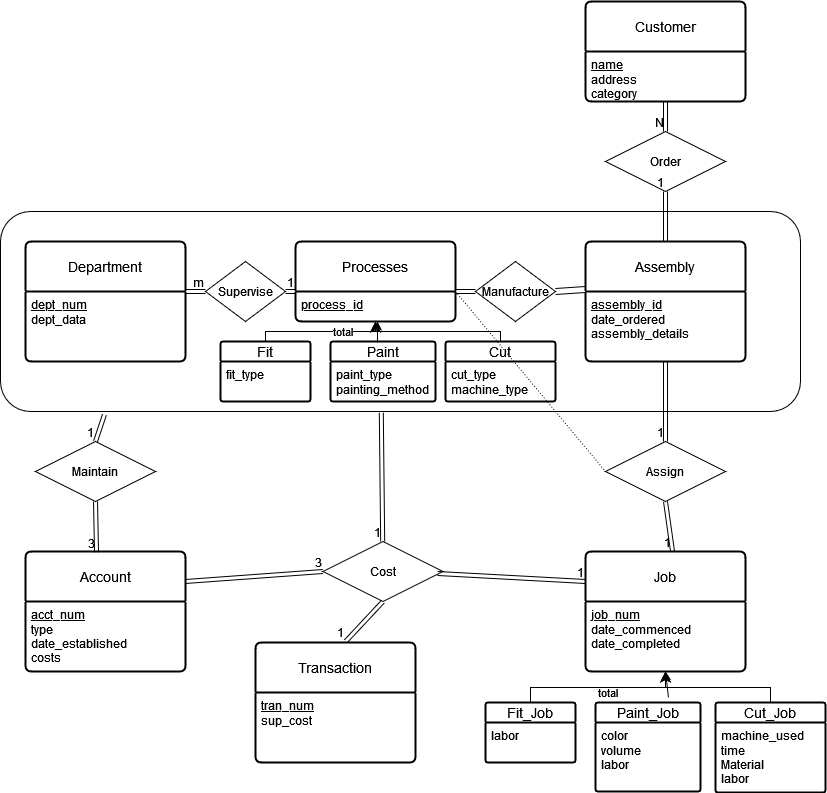
\includegraphics[width=\textwidth]{Project.png}
\newpage

\section{Relational Database Schema}

\indent Here are my schema:

Process(\underline{process\_id},process\_data)

Assemblies(\underline{ass\_id},date, ass\_details)

Create(\underline{process\_id},\underline{ass\_id})

Customer(\underline{name},address, category)

Orders(\underline{name},\underline{ass\_id})

Department(\underline{dept\_num},dept\_data)

Supervises(\underline{dept\_num},\underline{process\_id})

Fit(\underline{process\_id}, fit\_type)

Paint(\underline{process\_id}, paint\_type, painting\_method)

Cut(\underline{process\_id},cutting\_type, machine\_type)

Account(\underline{type}, \underline{acct\_id})

Job(\underline{process\_id}, \underline{ass\_id}, \underline{job\_num}, job\_date\_commence, job\_date\_end)


Costs(\underline{job\_num},\underline{type}, \underline{acct\_id},\underline{process\_id}, \underline{ass\_id})

Fit\_Job(\underline{process\_id}, \underline{ass\_id}, \underline{job\_num}, labor)

Paint\_Job(\underline{process\_id}, \underline{ass\_id}, \underline{job\_num},color,volume, labor)

Cut\_Job(\underline{process\_id}, \underline{ass\_id}, \underline{job\_num}, machine\_type, time, material, labor)

\newpage
\section{Storage}

\begin{tabular}{|p{.75in}|p{.75in}|p{.75in}|p{.65in}|p{.75in}|p{1.75in}|}\hline
Table Name & Query Number and Type & Search Key& Query Frequency& Selected File Organization & Justification\\ \hline\hline
Customer & 1 Insertion & name & 30/Day & heap tree on name & At the moment adding lots of data and not accessing it directly often\\ \hline 
Department & 2 Insertion& dept\_num & infrequent & Sequential on dept\_num & Since this data is added infrequently but referenced by other tables often, sequential insertion seems appropriate.\\ \hline
Process (and sub categories)& 3 Insertion & process\_id,  (sub category info) & infrequent & Sequential on process\_id (and sub category id)&  Infrequent insertion but often called\\ \hline
Supervises & 3 Insertion & process\_id and dept\_num & infrequent & Sequential on process\_id &Infrequent insertion but called often on process\_id\\\hline
Orders & 4 Insertion & name, ass\_id& 40/Day&dynamic hash on name and ass\_id& This is a lot of orders to create each day.  These will need to be joined with other tables frequently as is happening in our insertion so it is important to be easily accessible  \\ \hline
Create  & 4 Insertion & process\_id and ass\_id &40/Day &dynamic hash on process\_id and ass\_id & Frequent insertion with joins on other tables            \\ \hline
Account & 5 Insertion & type and acct\_id & 10/Day & Multitable clustering with type for clustering and acct\_id sequential& This structure will make for fast access later and there is a fair amount of additions here.\\ \hline
\end{tabular}
\newpage
\begin{tabular}{|p{.75in}|p{.75in}|p{.75in}|p{.65in}|p{.75in}|p{1.75in}|}\hline
Table Name & Query Number and Type & Search Key& Query Frequency& Selected File Organization & Justification\\ \hline\hline
Job & 6 Insertion & job\_num        \\ \hline

Job & 7 Random Search (Insertion of job\_date\_end) & job\_num & 50/Day & $B$ tree on job\_num  &To enter completion data, you'll need a random search on job\_num.  $B$ tree will be an efficient storage for all these records \\ \hline

Customer & 12 Range Search & name (in order) by category &100/Day & Multitable Clustering with category for clustering and name stored in a $B^+$ tree& Since this data is accessed often this table should be pre-built.  New customers are added often so $B^+$ tree storage on name will be most efficient within this multitable\\\hline
\end{tabular}

\end{document}